\section{Introduction}

A store can preserve a rule's text while losing the model behavior that rule taught.
In a joint prompt, appending three entries for unrelated keys does not overwrite an old record, but it can change how the reader uses that record.
Suppose each new entry is safe alone and every pair is safe, yet the triple flips the old answer.
An audit that checks at most two entries at a time would approve that triple.
The database analogy is write skew: changes valid in isolation can violate a shared invariant when combined~\citep{berenson1995}.
Here writes are prompt entries, not concurrent transactions, and the invariant is a model prediction rather than a database constraint.

A flip is not, on its own, evidence of a three-way interaction.
Three additive losses can exhaust a margin even if no two do.
Conversely, a nonzero three-way coefficient need not cause a flip, and can arise from a nonlinear response to rule count alone.
An earlier routing probe found that many unrelated records reduce old-rule margins, but did not vary all subsets at matched token positions~\citep{cldilution,clreanalysis}.
This leaves open whether the loss needs a particular combination of lessons.

We separate these claims using a complete three-lesson factorial with a frozen reader.
All eight contexts retain the old rule, token length, positions, and printed queue labels.
We check the old answer against every rival and estimate the three-way contrast against a fixed rival.
A pairwise extrapolation tests whether lower-order evidence would already forecast the flip; a separate count fit and disjoint replacement triples test whether the remaining variation is distinctive.
In \holdoutN{} held-out stores, we find one case that both forecasts miss; it vanishes under a second phrasing (\cref{fig:factorial}).
The goal is a screening decision on this setting, not an estimate of write skew across learners.

\begin{figure}[t]
\centering
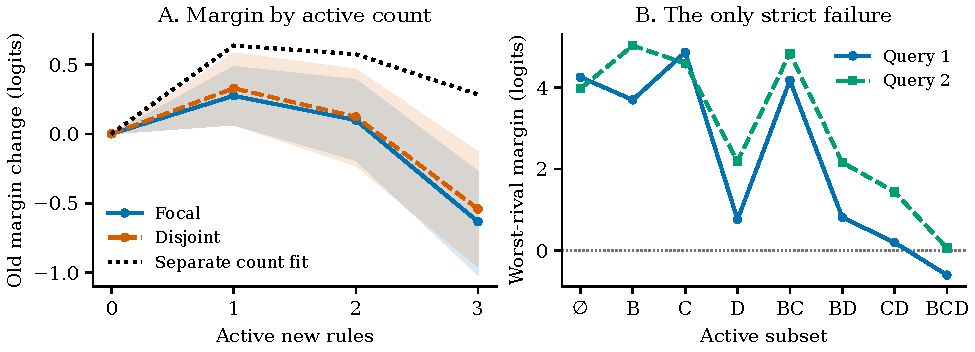
\includegraphics[width=\linewidth]{factorial.pdf}
\caption{\textbf{The only strict failure depends on the wording of the query.}
Left: mean change from the no-new-rule cell in the fixed-rival margin by active rule count.
Points average the available subsets within each of \holdoutN{} held-out stores; bands are store-bootstrap 95\% intervals.
The count fit uses \fitN{} separate stores.
Right: each point is the worst-rival margin for one subset of the sole strict witness (store \witnessSeed{}).
Below zero the old rule is no longer the top prediction. Query 2 keeps the identical store and changes only the question wording.}
\label{fig:factorial}
\end{figure}
